\chapter{功能介绍}

\section{进程管理}

进程模块总的可以分为进程创建与结束、进程调度、进程等待机制、杀死进程等四个方面的功能。

进程创建用于在系统中创建新的进程,而新创建的进程会自动设定为当前进程子进程。进程结束为在进程结束之后将退出系统时进行的操作。可支持按照指定优先级创建新进程。

进程调度用于对系统中所同时存在的多个进程进行调度,合理分配硬件资源。

进程等待机制用于协调进程之间的同步,通过进程等待机制可以使得将一个进程挂起,而等到另一个指定进程完成之后才将挂起进程恢复执行。但在此机制中挂起进程与被等待进程之间必须满足父子关系。

杀死进程使得用户或者程序可以强制结束特定进程的执行,以灵活管理进程。

其中提供接口供用户使用的指令有:


\begin{table}[H]
  \centering
  \caption{进程模块提供的用户指令}
  \includegraphics[scale=0.8]{process/img/用户指令.pdf}
\end{table}


\section{进程管理}

进程模块总的可以分为进程创建与结束、进程调度、进程等待机制、杀死进程等四个方面的功能。

进程创建用于在系统中创建新的进程,而新创建的进程会自动设定为当前进程子进程。进程结束为在进程结束之后将退出系统时进行的操作。可支持按照指定优先级创建新进程。

进程调度用于对系统中所同时存在的多个进程进行调度,合理分配硬件资源。

进程等待机制用于协调进程之间的同步,通过进程等待机制可以使得将一个进程挂起,而等到另一个指定进程完成之后才将挂起进程恢复执行。但在此机制中挂起进程与被等待进程之间必须满足父子关系。

杀死进程使得用户或者程序可以强制结束特定进程的执行,以灵活管理进程。

其中提供接口供用户使用的指令有:


\begin{table}[H]
  \centering
  \caption{进程模块提供的用户指令}
  \includegraphics[scale=0.8]{process/img/用户指令.pdf}
\end{table}


\section{进程管理}

进程模块总的可以分为进程创建与结束、进程调度、进程等待机制、杀死进程等四个方面的功能。

进程创建用于在系统中创建新的进程,而新创建的进程会自动设定为当前进程子进程。进程结束为在进程结束之后将退出系统时进行的操作。可支持按照指定优先级创建新进程。

进程调度用于对系统中所同时存在的多个进程进行调度,合理分配硬件资源。

进程等待机制用于协调进程之间的同步,通过进程等待机制可以使得将一个进程挂起,而等到另一个指定进程完成之后才将挂起进程恢复执行。但在此机制中挂起进程与被等待进程之间必须满足父子关系。

杀死进程使得用户或者程序可以强制结束特定进程的执行,以灵活管理进程。

其中提供接口供用户使用的指令有:


\begin{table}[H]
  \centering
  \caption{进程模块提供的用户指令}
  \includegraphics[scale=0.8]{process/img/用户指令.pdf}
\end{table}




\chapter{详细设计}

\section{进程管理: 多级反馈队列}

\subsection{进程数据结构}

\subsubsection{\texttt{task\_struct}结构}

\texttt{task\_struct}结构即为进程控制块,是进程模块中最主要的结构。本系统中的\texttt{task\_struct}设计参考Linux系统中的进程控制块结构。结合本操作系统的实际需要对Linux的进程控制块结构进行了删减和修改,使之更符合本系统的需要。

\texttt{task\_struct}结构具体信息见下图。

\begin{lstlisting}[caption=\texttt{task\_struct}结构]
//进程PCB结构,保存进程状态等相关信息
struct task_struct {
    pid_t pid;                             // 进程pid号
    unsigned char name[TASK_NAME_LEN];     // 进程名
    pid_t parent;                          // 父进程pid号
    int ASID;                              // 进程地址空间id号
    int state;                             // 进程状态

    unsigned int time_cnt;                 // 进程所拥有的时间片
    unsigned int priority;                 // 进程的优先级  

    struct regs_context context;           // 进程寄存器信息
    struct mm_struct *mm;                  // 进程地址空间结构指针
    FILE *task_files;                      // 进程打开文件指针

    struct list_head sched_list;           // 用于进程调度
    struct list_head task_list;            // 用于进程链表
};
\end{lstlisting}

\newpage
\subsubsection{\texttt{task\_union}结构}

此结构利用C语言中的union关键字,巧妙地将进程的内核栈和进程控制块合并在一起进行存储,设计思想同样是源于Linux系统。

\texttt{task\_union}结构具体信息见下图。


\begin{lstlisting}[caption=\texttt{task\_union}数据结构]
union task_union {
    struct task_struct task;                        //进程控制块
    unsigned char kernel_stack[KERNEL_STACK_SIZE];  //进程的内核栈
};
\end{lstlisting}

\subsubsection{\texttt{regs\_context}结构}

\texttt{regs\_context}结构用于存储进程的寄存器信息,属于进程模块的辅助结构。主要用于当系统中出现进程调度、进程退出等需要进行进程切换操作的情况时保存进程的寄存器信息,其实也就是在保存进程的状态信息,以便在进程再次恢复执行时能够从一个正确的状态启动。

而在该结构中,不只是保存通用寄存器内容,也会对CP0协处理器中的EPC寄存器内容进行保存,而EPC寄存器中所存储的正是进程重新开始执行的指令地址。

\texttt{regs\_context}结构具体信息见下图。

\begin{lstlisting}[caption=\texttt{regs\_context}结构]
//寄存器信息结构,主要用于进程调度时的进程切换
struct regs_context {
    unsigned int epc;
    unsigned int at;
    unsigned int v0, v1;
    unsigned int a0, a1, a2, a3;
    unsigned int t0, t1, t2, t3, t4, t5, t6, t7;
    unsigned int s0, s1, s2, s3, s4, s5, s6, s7;
    unsigned int t8, t9;
    unsigned int hi, lo;
    unsigned int gp, sp, fp, ra;
};
\end{lstlisting}

\subsubsection{\texttt{ready\_list}结构}

\texttt{ready\_list}结构用于存储进程的多级反馈就绪队列,属于进程模块的辅助结构。主要用于管理进程的就绪队列,在进程调度、进程退出等需要进行进程切换操作的情况时存储处于就绪队列的进程,不同的队列代表不同的优先级的就绪队列,按照数组地址顺序匹配优先级大小排列,以便于查找在进程调度遍历多级就绪队列查找高优先级的进程。

\texttt{ready\_list}结构具体信息见下图。

\begin{lstlisting}[caption=\texttt{ready\_list}结构]
struct ready_list {
    int size;                           //记录当前队列长度
    struct list_head head;              //记录队列的头部节点
};
\end{lstlisting}

\subsubsection{其他与进程有关的全局链表}

本操作系统中以下的全局链表采用Linux中的\texttt{struct list\_head}结构。



\begin{table}[H]
  \centering
  \caption{进程有关全局链表}
  \begin{tabular}{|c|c|}
  \hline
  链表名 & 用途 \\
  \hline
  \texttt{total\_tasks}  & 系统中的全部进程 \\
  \hline
  \texttt{total\_wait}   & 系统中的所有等待进程 \\
  \hline
  \texttt{total\_exited} & 系统中的所有结束或未分配进程 \\
  \hline
  \end{tabular}
\end{table}


\subsection{进程创建}

用户输入的\texttt{execprio},\texttt{execk},\texttt{execwait}等不同的进程创建指令,都统一调用\texttt{exec\_from\_kernel}函数。在\texttt{exec\_from\_kernel}函数中调用\texttt{task\_create}函数创建新的进程,并且提供给\texttt{task\_create}函数一个函数指针,作为进程开始执行的入口地址,默认设置新创建进程的入口地址为内核函数\texttt{runprog}。

而在\texttt{task\_create}函数中,首先我们为新创建进程分配一个新的pid号,创建相应的\texttt{task\_struct}结构,以及初始化结构内部必要的信息。为新建进程分配资源,建立对应的虚拟地址空间即\texttt{mm\_struct}结构,初始化进程打开文件。其次,我们设置进程的状态信息,比如堆栈、进程入口、进程状态,根据优先级设置默认分配的时间片,并设置完毕后将新创建的进程加入就绪队列。

在\texttt{init\_kernel}函数中会初始化进程相关的部分,idle进程总是第一个被创建的,pid为0的进程。
\texttt{kernel shell}进程是在\texttt{init\_kernel()}中调用\texttt{task\_create()}第二个被创建的,pid为1的进程。

进程创建过程的层次结构如下。

\begin{table}[H]
  \centering
  \caption{创建进程过程的层次结构}
  \includegraphics[scale=0.8]{process/img/创建进程过程的层次结构.pdf}\\
  {注:蓝色部分表示在新创建进程运行的部分}
\end{table}

\begin{table}[H]
  \centering
  \caption{\texttt{task\_create}函数处理层次结构}
  \includegraphics[scale=0.8]{process/img/task_create().pdf}
\end{table}


\subsection{进程退出}

首先会调用唤醒父进程函数\texttt{wakeup\_parent}函数,检查要退出进程的父进程是否在等待它,如果是,则唤醒父进程,使父进程恢复到可执行状态。然后将要退出进程的状态更改为终止状态,并且释放分配给进程的一些资源、如关闭已打开文件、释放\texttt{mm\_struct}结构(描述进程地址空间的结构)等,最后将对应进程移出多级就绪队列并放入进程结束链表中,并且通过调度算法寻找下一个可执行的进程。在每次进程调度发生时,会对进程结束链表进行清理,释放资源。

进程退出过程的层次结构如下。

\begin{table}[H]
  \centering
  \caption{\texttt{pc\_exit}函数处理层次结构}
  \includegraphics[scale=0.8]{process/img/pc_exit.pdf}
\end{table}


\subsection{进程调度}

在本操作系统中采用的调度算法是以多级反馈队列调度算法为基础进行修改的。

初始化后,我们的多级就绪队列中有初始的idle进程、和kernel shell进程,idle进程和kernel shell进程也有默认的时间片,如果不创建其他进程时,kernel shell进程将会不断地和idle进程进行调度切换。

多级就绪队列的级数可以使用宏任意设定,不影响调度算法的核心部分。调度算法的核心是在当前进程时间片未用完时,可以被更高优先级的进程实时抢占,如果当前进程的时间片已用完,将会在多级就绪队列中找到下一个不为当前进程的可执行的进程执行,如果没有比当前进程更高优先级的进程,则会寻找比当前进程优先级更低的进程,如果比当前优先级更低的进程只有idle进程(默认设为最低优先级),那么将会执行idle进程。当然,如果仍存在比idle进程优先级更高的进程(至少有kernel shell进程),idle进程执行时将会重新被抢占。

在找到下一个要执行的进程后,就只需要通过进程切换操作将寄存器中的信息更新为新的要执行的进程的信息即可开始新的进程的执行。

\begin{table}[H]
  \centering
  \caption{进程调度的层次结构}
  \includegraphics[scale=0.8]{process/img/pc_schedule.pdf}
\end{table}



\subsection{进程等待机制}

本操作系统中会引入进程等待机制,主要是用于实现进程之间的同步,使得父进程可以挂起以等待子进程执行完毕之后再继续执行。进程等待机制的实现主要依赖于两个函数\texttt{wait\_pid()}和\texttt{wakeup\_parent()}。

\texttt{wait\_pid()} 函数由父进程系统调用,参数为父进程所要等待的子进程的pid号。该函数会将父进程的状态修改为等待状态,并将其从从调度链表中移除而添加到进程等待链表中。然后通过调用进程调度算法选取下一个要执行的进程,并将下一个要执行的进程的上下文信息加载到寄存器中,即完成等待子进程操作。

而\texttt{wakeup\_parent()}函数由子进程在进程退出时系统调用的\texttt{pc\_exit()}函数中调用。该函数会首先检查当前进程的父进程是否在等待它,如果是的话,则会将父进程的状态修改为可执行状态,并将其从进程等待链表中移除而加入到多级就绪队列中,将其放入后台多级队列中相应队列的开头位置,这样使得父进程可以在进程调度时相对于同级队列中的进程优先被调度。

\subsection{kill进程}

本操作系统实现kill进程系统调用,主要是为了保证系统/用户对进程管理拥有比较大的自由度,使得系统/用户可以通过提供进程pid号对进程进行杀死操作。

当调用kill进程系统调用的\texttt{pc\_kill()}时,首先会判断要杀死的进程是否是不能杀死的进程以及所提供的进程pid号是否合法,如果合法,则将进程的状态更改为进程结束状态,释放分配给进程的资源,并将进程从调度链表或等待链表中移除而放入进程结束链表中,而进程结束链表会在进程调度发生时进行清理操作,释放相关资源。

\section{进程管理:UC/OS II}

由于进程部分总体工作量相对较少,又因为在实验课上提及的uC/OS II(Micro Control Operation System Two)系统非常有特点,因此在进程部分也尝试移植了该系统的任务管理部分。

采用的调度算法参考于uC/OS II(Micro Control Operation System Two)系统。它是一个可以基于ROM运行的、可裁减的、抢占式、实时多任务内核,具有高可移植性,特别适合于微处理器和控制器,是和很多商业操作系统性能相当的实时操作系统。它可以简单地视为是一个多任务调度器,在这个任务调度器之上完善并添加了和多任务操作系统相关的系统服务,比如信号量等。uC/OS II绝大部分代码使用C语言编写,CPU硬件相关部分是使用汇编语言编写的,其源代码公开。

在其任务调度部分,有许多有意思的特点,区别于我们之前在课堂上学习到的调度算法,比如使用优先级而不是进程pid来唯一标示进程,存在优先级继承机制,任务调度和事件机制的结合等。在这里,我们只移植了较为基础的纯粹的任务调度部分。

同时,进程创建和进程退出部分,一些数据结构和我们上述调度算法大同小异,接下来我们只重点阐述不同的部分。


\subsection{进程数据结构}

\subsubsection{\texttt{task\_struct}结构}

区别于之前的调度算法,uC/OS II中不是通过pid来唯一标示一个进程,而是使用优先级,每一个任务处于一个不同的优先级,并有一张任务就绪表来管理所有就绪的任务,为了提高效率,很多的操作都是通过位运算来进行的,优先级使用8位数字保存,也因此在该系统中最多含有64个任务(64个不同的优先级)。为了位运算的方便,参考该系统,我们也将优先级拆分为高位和低位分开保存。

\texttt{task\_struct}结构中最重点的部分如下图。

\begin{lstlisting}[caption=\texttt{task\_struct}数据结构]
unsigned char prio; /* task priority (hightest = 0) */
unsigned char x;/* Bit position in group corresponding to task priority */
unsigned char y;/* Index in ready table corresponding to task priority */
unsigned char bit_x;/* Bit mask to access bit position in ready table */        
unsigned char bit_y;/* Bit mask to access bit position in ready group */                       
\end{lstlisting}


\subsubsection{任务就绪表}

不同于我们之前的调度算法,或者是Linux/Windows的调度算法,该系统使用数组来管理所有的就绪任务。此任务就绪表用于管理就绪任务。

任务就绪表的定义如下图。

\begin{lstlisting}[caption=任务就绪表定义]
unsigned char rdy_group;  /* Ready list group  */
unsigned char rdy_table[OS_RDY_TBL_SIZE];
/* Table of tasks which are ready to run */
\end{lstlisting}


\subsubsection{任务控制块和就绪表的关联}

8位优先级按照小端保存时, 分别为D7, D6, D5, D4, D3, D2,D1, D0。在uC/OS II中最多64个优先级,即优先级的最大数值为\texttt{00111111},仅使用了6位数字表示(最大数值的优先级是最低优先级,0u是最高优先级)。所以任务控制块中的y表示任务优先级的高3位(D5, D4, D3),指明\texttt{rdy\_table}的下标,即\texttt{rdy\_group}的数据位。任务控制块中的x表示任务优先级的低三位(D2, D1, D0),指明\texttt{rdy\_table[y]}中的哪一位数据位。\texttt{bit\_y}和\texttt{bit\_x}主要是为了寻找最高优先级时匹配使用。

相应变量的计算方式如下图。


\begin{lstlisting}[caption=相关位运算]
ptcb->y = (unsigned char)(prio >> 3);
ptcb->x = (unsigned char)(prio & 0x07);
ptcb->bit_y = (unsigned char)(1 << ptcb->y);
ptcb->bit_x = (unsigned char)(1 << ptcb->x);
\end{lstlisting}


\subsubsection{\texttt{map\_table}表}
用于寻找最高优先级任务时进行匹配,找出目标任务的核心算法在于确定某数值为1的最低位(每个任务具有不同的优先级),uC/OS II中的具体实现是 ,借助\texttt{map\_table},通过高效的位运算完成。

\texttt{map\_table}表的结构如下图。

\begin{lstlisting}[caption=\texttt{map\_table}表]
unsigned char const  map_table[256] = {
  0u, 0u, 1u, 0u, 2u, 0u, 1u, 0u, 3u, 0u, 1u, 0u, 2u, 0u, 1u, 0u, 
  /* 0x00 to 0x0F */
  4u, 0u, 1u, 0u, 2u, 0u, 1u, 0u, 3u, 0u, 1u, 0u, 2u, 0u, 1u, 0u,
  /* 0x10 to 0x1F */
  5u, 0u, 1u, 0u, 2u, 0u, 1u, 0u, 3u, 0u, 1u, 0u, 2u, 0u, 1u, 0u, 
  /* 0x20 to 0x2F */
  4u, 0u, 1u, 0u, 2u, 0u, 1u, 0u, 3u, 0u, 1u, 0u, 2u, 0u, 1u, 0u, 
  /* 0x30 to 0x3F */
  6u, 0u, 1u, 0u, 2u, 0u, 1u, 0u, 3u, 0u, 1u, 0u, 2u, 0u, 1u, 0u, 
  /* 0x40 to 0x4F */
  4u, 0u, 1u, 0u, 2u, 0u, 1u, 0u, 3u, 0u, 1u, 0u, 2u, 0u, 1u, 0u, 
  /* 0x50 to 0x5F */
  5u, 0u, 1u, 0u, 2u, 0u, 1u, 0u, 3u, 0u, 1u, 0u, 2u, 0u, 1u, 0u, 
  /* 0x60 to 0x6F */
  4u, 0u, 1u, 0u, 2u, 0u, 1u, 0u, 3u, 0u, 1u, 0u, 2u, 0u, 1u, 0u, 
  /* 0x70 to 0x7F */
  7u, 0u, 1u, 0u, 2u, 0u, 1u, 0u, 3u, 0u, 1u, 0u, 2u, 0u, 1u, 0u, 
  /* 0x80 to 0x8F */
  4u, 0u, 1u, 0u, 2u, 0u, 1u, 0u, 3u, 0u, 1u, 0u, 2u, 0u, 1u, 0u,
  /* 0x90 to 0x9F */
  5u, 0u, 1u, 0u, 2u, 0u, 1u, 0u, 3u, 0u, 1u, 0u, 2u, 0u, 1u, 0u, 
  /* 0xA0 to 0xAF */
  4u, 0u, 1u, 0u, 2u, 0u, 1u, 0u, 3u, 0u, 1u, 0u, 2u, 0u, 1u, 0u,
  /* 0xB0 to 0xBF */
  6u, 0u, 1u, 0u, 2u, 0u, 1u, 0u, 3u, 0u, 1u, 0u, 2u, 0u, 1u, 0u,
  /* 0xC0 to 0xCF */
  4u, 0u, 1u, 0u, 2u, 0u, 1u, 0u, 3u, 0u, 1u, 0u, 2u, 0u, 1u, 0u,
  /* 0xD0 to 0xDF */
  5u, 0u, 1u, 0u, 2u, 0u, 1u, 0u, 3u, 0u, 1u, 0u, 2u, 0u, 1u, 0u,
  /* 0xE0 to 0xEF */
  4u, 0u, 1u, 0u, 2u, 0u, 1u, 0u, 3u, 0u, 1u, 0u, 2u, 0u, 1u, 0u 
  /* 0xF0 to 0xFF */
};
\end{lstlisting}




\subsection{任务管理操作}

\subsubsection{登记就绪任务}

当某个任务处于就绪状态时,系统就将该任务登记在任务就绪表中,即在该任务优先级对应的任务就绪表中的位置设置值为1。
对应的位操作如下图。

\begin{lstlisting}[caption=登记就绪任务操作]
rdy_group |= ptcb->bit_y;
rdy_table[y] |= ptcb->bit_x;
\end{lstlisting}


\subsubsection{注销就绪任务}

当某个任务处于就绪状态时,系统就将该任务在任务就绪表中注销,即在该任务优先级对应的任务就绪表中的位置重置值为0。
对应的位操作如下图。

\begin{lstlisting}[caption=注销就绪任务操作]
unsigned char y;
y = current_task->y;
rdy_table[y] &= ~current_task->bit_x;   // set the bit in rdy_table[y] zero
if (rdy_table[y] == 0x00) {             // no ready task
  rdy_group &= ~current_task->bit_y;    // set the bit in rdy_group zero
}
\end{lstlisting}

\subsubsection{寻找最高优先级任务}

用于寻找最高优先级任务时进行匹配,找出目标任务的核心算法在于确定某数值为1的最低位(每个任务具有不同的优先级)。本质上就是哈希算法。
对应的位操作如下图。

\begin{lstlisting}[caption=寻找最高优先级任务操作]
unsigned char y;
y = map_table[rdy_group]; // group the highest task in
prio_highest_rdy = (unsigned char)((y << 3) + map_table[rdy_table[y]]); 
// which bit in group
\end{lstlisting}



\subsection{进程调度}

为了简化系统设计,在移植部分没有修改原有系统的中断触发的底层部分,进程调度发生的情况如下:

一方面是进程级的上下文切换,具有高优先级的进程因为需要某种临界资源,主动请求挂起,让出处理器,此时发生进程调度,执行处于就绪状态的低优先级进程。

另一方面是中断级的上下文切换,具有高优先级的进程时间片用完,在时钟中断的处理程序中,内核发现高优先级的进程重新获得了执行条件,则从中断态直接切换到高优先级的进行执行。

我们使用一个调度链表管理所有任务,初始化后含有idle进程和kernel shell进程。调度的工作主要分为两部分:最高优先级进程的寻找和进程切换。最高优先级进程的寻找我们通过建立就绪进程表,使用数组管理实现。在进程切换时,先使用变量记录当前最高就绪任务的结点,然后调用相关函数进行切换,将寄存器中的信息更新为新的要执行进程的信息即可开始新的进程的执行。同时更新任务就绪表中的操作。




\section{进程管理: 多级反馈队列}

\subsection{进程数据结构}

\subsubsection{\texttt{task\_struct}结构}

\texttt{task\_struct}结构即为进程控制块,是进程模块中最主要的结构。本系统中的\texttt{task\_struct}设计参考Linux系统中的进程控制块结构。结合本操作系统的实际需要对Linux的进程控制块结构进行了删减和修改,使之更符合本系统的需要。

\texttt{task\_struct}结构具体信息见下图。

\begin{lstlisting}[caption=\texttt{task\_struct}结构]
//进程PCB结构,保存进程状态等相关信息
struct task_struct {
    pid_t pid;                             // 进程pid号
    unsigned char name[TASK_NAME_LEN];     // 进程名
    pid_t parent;                          // 父进程pid号
    int ASID;                              // 进程地址空间id号
    int state;                             // 进程状态

    unsigned int time_cnt;                 // 进程所拥有的时间片
    unsigned int priority;                 // 进程的优先级  

    struct regs_context context;           // 进程寄存器信息
    struct mm_struct *mm;                  // 进程地址空间结构指针
    FILE *task_files;                      // 进程打开文件指针

    struct list_head sched_list;           // 用于进程调度
    struct list_head task_list;            // 用于进程链表
};
\end{lstlisting}

\newpage
\subsubsection{\texttt{task\_union}结构}

此结构利用C语言中的union关键字,巧妙地将进程的内核栈和进程控制块合并在一起进行存储,设计思想同样是源于Linux系统。

\texttt{task\_union}结构具体信息见下图。


\begin{lstlisting}[caption=\texttt{task\_union}数据结构]
union task_union {
    struct task_struct task;                        //进程控制块
    unsigned char kernel_stack[KERNEL_STACK_SIZE];  //进程的内核栈
};
\end{lstlisting}

\subsubsection{\texttt{regs\_context}结构}

\texttt{regs\_context}结构用于存储进程的寄存器信息,属于进程模块的辅助结构。主要用于当系统中出现进程调度、进程退出等需要进行进程切换操作的情况时保存进程的寄存器信息,其实也就是在保存进程的状态信息,以便在进程再次恢复执行时能够从一个正确的状态启动。

而在该结构中,不只是保存通用寄存器内容,也会对CP0协处理器中的EPC寄存器内容进行保存,而EPC寄存器中所存储的正是进程重新开始执行的指令地址。

\texttt{regs\_context}结构具体信息见下图。

\begin{lstlisting}[caption=\texttt{regs\_context}结构]
//寄存器信息结构,主要用于进程调度时的进程切换
struct regs_context {
    unsigned int epc;
    unsigned int at;
    unsigned int v0, v1;
    unsigned int a0, a1, a2, a3;
    unsigned int t0, t1, t2, t3, t4, t5, t6, t7;
    unsigned int s0, s1, s2, s3, s4, s5, s6, s7;
    unsigned int t8, t9;
    unsigned int hi, lo;
    unsigned int gp, sp, fp, ra;
};
\end{lstlisting}

\subsubsection{\texttt{ready\_list}结构}

\texttt{ready\_list}结构用于存储进程的多级反馈就绪队列,属于进程模块的辅助结构。主要用于管理进程的就绪队列,在进程调度、进程退出等需要进行进程切换操作的情况时存储处于就绪队列的进程,不同的队列代表不同的优先级的就绪队列,按照数组地址顺序匹配优先级大小排列,以便于查找在进程调度遍历多级就绪队列查找高优先级的进程。

\texttt{ready\_list}结构具体信息见下图。

\begin{lstlisting}[caption=\texttt{ready\_list}结构]
struct ready_list {
    int size;                           //记录当前队列长度
    struct list_head head;              //记录队列的头部节点
};
\end{lstlisting}

\subsubsection{其他与进程有关的全局链表}

本操作系统中以下的全局链表采用Linux中的\texttt{struct list\_head}结构。



\begin{table}[H]
  \centering
  \caption{进程有关全局链表}
  \begin{tabular}{|c|c|}
  \hline
  链表名 & 用途 \\
  \hline
  \texttt{total\_tasks}  & 系统中的全部进程 \\
  \hline
  \texttt{total\_wait}   & 系统中的所有等待进程 \\
  \hline
  \texttt{total\_exited} & 系统中的所有结束或未分配进程 \\
  \hline
  \end{tabular}
\end{table}


\subsection{进程创建}

用户输入的\texttt{execprio},\texttt{execk},\texttt{execwait}等不同的进程创建指令,都统一调用\texttt{exec\_from\_kernel}函数。在\texttt{exec\_from\_kernel}函数中调用\texttt{task\_create}函数创建新的进程,并且提供给\texttt{task\_create}函数一个函数指针,作为进程开始执行的入口地址,默认设置新创建进程的入口地址为内核函数\texttt{runprog}。

而在\texttt{task\_create}函数中,首先我们为新创建进程分配一个新的pid号,创建相应的\texttt{task\_struct}结构,以及初始化结构内部必要的信息。为新建进程分配资源,建立对应的虚拟地址空间即\texttt{mm\_struct}结构,初始化进程打开文件。其次,我们设置进程的状态信息,比如堆栈、进程入口、进程状态,根据优先级设置默认分配的时间片,并设置完毕后将新创建的进程加入就绪队列。

在\texttt{init\_kernel}函数中会初始化进程相关的部分,idle进程总是第一个被创建的,pid为0的进程。
\texttt{kernel shell}进程是在\texttt{init\_kernel()}中调用\texttt{task\_create()}第二个被创建的,pid为1的进程。

进程创建过程的层次结构如下。

\begin{table}[H]
  \centering
  \caption{创建进程过程的层次结构}
  \includegraphics[scale=0.8]{process/img/创建进程过程的层次结构.pdf}\\
  {注:蓝色部分表示在新创建进程运行的部分}
\end{table}

\begin{table}[H]
  \centering
  \caption{\texttt{task\_create}函数处理层次结构}
  \includegraphics[scale=0.8]{process/img/task_create().pdf}
\end{table}


\subsection{进程退出}

首先会调用唤醒父进程函数\texttt{wakeup\_parent}函数,检查要退出进程的父进程是否在等待它,如果是,则唤醒父进程,使父进程恢复到可执行状态。然后将要退出进程的状态更改为终止状态,并且释放分配给进程的一些资源、如关闭已打开文件、释放\texttt{mm\_struct}结构(描述进程地址空间的结构)等,最后将对应进程移出多级就绪队列并放入进程结束链表中,并且通过调度算法寻找下一个可执行的进程。在每次进程调度发生时,会对进程结束链表进行清理,释放资源。

进程退出过程的层次结构如下。

\begin{table}[H]
  \centering
  \caption{\texttt{pc\_exit}函数处理层次结构}
  \includegraphics[scale=0.8]{process/img/pc_exit.pdf}
\end{table}


\subsection{进程调度}

在本操作系统中采用的调度算法是以多级反馈队列调度算法为基础进行修改的。

初始化后,我们的多级就绪队列中有初始的idle进程、和kernel shell进程,idle进程和kernel shell进程也有默认的时间片,如果不创建其他进程时,kernel shell进程将会不断地和idle进程进行调度切换。

多级就绪队列的级数可以使用宏任意设定,不影响调度算法的核心部分。调度算法的核心是在当前进程时间片未用完时,可以被更高优先级的进程实时抢占,如果当前进程的时间片已用完,将会在多级就绪队列中找到下一个不为当前进程的可执行的进程执行,如果没有比当前进程更高优先级的进程,则会寻找比当前进程优先级更低的进程,如果比当前优先级更低的进程只有idle进程(默认设为最低优先级),那么将会执行idle进程。当然,如果仍存在比idle进程优先级更高的进程(至少有kernel shell进程),idle进程执行时将会重新被抢占。

在找到下一个要执行的进程后,就只需要通过进程切换操作将寄存器中的信息更新为新的要执行的进程的信息即可开始新的进程的执行。

\begin{table}[H]
  \centering
  \caption{进程调度的层次结构}
  \includegraphics[scale=0.8]{process/img/pc_schedule.pdf}
\end{table}



\subsection{进程等待机制}

本操作系统中会引入进程等待机制,主要是用于实现进程之间的同步,使得父进程可以挂起以等待子进程执行完毕之后再继续执行。进程等待机制的实现主要依赖于两个函数\texttt{wait\_pid()}和\texttt{wakeup\_parent()}。

\texttt{wait\_pid()} 函数由父进程系统调用,参数为父进程所要等待的子进程的pid号。该函数会将父进程的状态修改为等待状态,并将其从从调度链表中移除而添加到进程等待链表中。然后通过调用进程调度算法选取下一个要执行的进程,并将下一个要执行的进程的上下文信息加载到寄存器中,即完成等待子进程操作。

而\texttt{wakeup\_parent()}函数由子进程在进程退出时系统调用的\texttt{pc\_exit()}函数中调用。该函数会首先检查当前进程的父进程是否在等待它,如果是的话,则会将父进程的状态修改为可执行状态,并将其从进程等待链表中移除而加入到多级就绪队列中,将其放入后台多级队列中相应队列的开头位置,这样使得父进程可以在进程调度时相对于同级队列中的进程优先被调度。

\subsection{kill进程}

本操作系统实现kill进程系统调用,主要是为了保证系统/用户对进程管理拥有比较大的自由度,使得系统/用户可以通过提供进程pid号对进程进行杀死操作。

当调用kill进程系统调用的\texttt{pc\_kill()}时,首先会判断要杀死的进程是否是不能杀死的进程以及所提供的进程pid号是否合法,如果合法,则将进程的状态更改为进程结束状态,释放分配给进程的资源,并将进程从调度链表或等待链表中移除而放入进程结束链表中,而进程结束链表会在进程调度发生时进行清理操作,释放相关资源。

\section{进程管理:UC/OS II}

由于进程部分总体工作量相对较少,又因为在实验课上提及的uC/OS II(Micro Control Operation System Two)系统非常有特点,因此在进程部分也尝试移植了该系统的任务管理部分。

采用的调度算法参考于uC/OS II(Micro Control Operation System Two)系统。它是一个可以基于ROM运行的、可裁减的、抢占式、实时多任务内核,具有高可移植性,特别适合于微处理器和控制器,是和很多商业操作系统性能相当的实时操作系统。它可以简单地视为是一个多任务调度器,在这个任务调度器之上完善并添加了和多任务操作系统相关的系统服务,比如信号量等。uC/OS II绝大部分代码使用C语言编写,CPU硬件相关部分是使用汇编语言编写的,其源代码公开。

在其任务调度部分,有许多有意思的特点,区别于我们之前在课堂上学习到的调度算法,比如使用优先级而不是进程pid来唯一标示进程,存在优先级继承机制,任务调度和事件机制的结合等。在这里,我们只移植了较为基础的纯粹的任务调度部分。

同时,进程创建和进程退出部分,一些数据结构和我们上述调度算法大同小异,接下来我们只重点阐述不同的部分。


\subsection{进程数据结构}

\subsubsection{\texttt{task\_struct}结构}

区别于之前的调度算法,uC/OS II中不是通过pid来唯一标示一个进程,而是使用优先级,每一个任务处于一个不同的优先级,并有一张任务就绪表来管理所有就绪的任务,为了提高效率,很多的操作都是通过位运算来进行的,优先级使用8位数字保存,也因此在该系统中最多含有64个任务(64个不同的优先级)。为了位运算的方便,参考该系统,我们也将优先级拆分为高位和低位分开保存。

\texttt{task\_struct}结构中最重点的部分如下图。

\begin{lstlisting}[caption=\texttt{task\_struct}数据结构]
unsigned char prio; /* task priority (hightest = 0) */
unsigned char x;/* Bit position in group corresponding to task priority */
unsigned char y;/* Index in ready table corresponding to task priority */
unsigned char bit_x;/* Bit mask to access bit position in ready table */        
unsigned char bit_y;/* Bit mask to access bit position in ready group */                       
\end{lstlisting}


\subsubsection{任务就绪表}

不同于我们之前的调度算法,或者是Linux/Windows的调度算法,该系统使用数组来管理所有的就绪任务。此任务就绪表用于管理就绪任务。

任务就绪表的定义如下图。

\begin{lstlisting}[caption=任务就绪表定义]
unsigned char rdy_group;  /* Ready list group  */
unsigned char rdy_table[OS_RDY_TBL_SIZE];
/* Table of tasks which are ready to run */
\end{lstlisting}


\subsubsection{任务控制块和就绪表的关联}

8位优先级按照小端保存时, 分别为D7, D6, D5, D4, D3, D2,D1, D0。在uC/OS II中最多64个优先级,即优先级的最大数值为\texttt{00111111},仅使用了6位数字表示(最大数值的优先级是最低优先级,0u是最高优先级)。所以任务控制块中的y表示任务优先级的高3位(D5, D4, D3),指明\texttt{rdy\_table}的下标,即\texttt{rdy\_group}的数据位。任务控制块中的x表示任务优先级的低三位(D2, D1, D0),指明\texttt{rdy\_table[y]}中的哪一位数据位。\texttt{bit\_y}和\texttt{bit\_x}主要是为了寻找最高优先级时匹配使用。

相应变量的计算方式如下图。


\begin{lstlisting}[caption=相关位运算]
ptcb->y = (unsigned char)(prio >> 3);
ptcb->x = (unsigned char)(prio & 0x07);
ptcb->bit_y = (unsigned char)(1 << ptcb->y);
ptcb->bit_x = (unsigned char)(1 << ptcb->x);
\end{lstlisting}


\subsubsection{\texttt{map\_table}表}
用于寻找最高优先级任务时进行匹配,找出目标任务的核心算法在于确定某数值为1的最低位(每个任务具有不同的优先级),uC/OS II中的具体实现是 ,借助\texttt{map\_table},通过高效的位运算完成。

\texttt{map\_table}表的结构如下图。

\begin{lstlisting}[caption=\texttt{map\_table}表]
unsigned char const  map_table[256] = {
  0u, 0u, 1u, 0u, 2u, 0u, 1u, 0u, 3u, 0u, 1u, 0u, 2u, 0u, 1u, 0u, 
  /* 0x00 to 0x0F */
  4u, 0u, 1u, 0u, 2u, 0u, 1u, 0u, 3u, 0u, 1u, 0u, 2u, 0u, 1u, 0u,
  /* 0x10 to 0x1F */
  5u, 0u, 1u, 0u, 2u, 0u, 1u, 0u, 3u, 0u, 1u, 0u, 2u, 0u, 1u, 0u, 
  /* 0x20 to 0x2F */
  4u, 0u, 1u, 0u, 2u, 0u, 1u, 0u, 3u, 0u, 1u, 0u, 2u, 0u, 1u, 0u, 
  /* 0x30 to 0x3F */
  6u, 0u, 1u, 0u, 2u, 0u, 1u, 0u, 3u, 0u, 1u, 0u, 2u, 0u, 1u, 0u, 
  /* 0x40 to 0x4F */
  4u, 0u, 1u, 0u, 2u, 0u, 1u, 0u, 3u, 0u, 1u, 0u, 2u, 0u, 1u, 0u, 
  /* 0x50 to 0x5F */
  5u, 0u, 1u, 0u, 2u, 0u, 1u, 0u, 3u, 0u, 1u, 0u, 2u, 0u, 1u, 0u, 
  /* 0x60 to 0x6F */
  4u, 0u, 1u, 0u, 2u, 0u, 1u, 0u, 3u, 0u, 1u, 0u, 2u, 0u, 1u, 0u, 
  /* 0x70 to 0x7F */
  7u, 0u, 1u, 0u, 2u, 0u, 1u, 0u, 3u, 0u, 1u, 0u, 2u, 0u, 1u, 0u, 
  /* 0x80 to 0x8F */
  4u, 0u, 1u, 0u, 2u, 0u, 1u, 0u, 3u, 0u, 1u, 0u, 2u, 0u, 1u, 0u,
  /* 0x90 to 0x9F */
  5u, 0u, 1u, 0u, 2u, 0u, 1u, 0u, 3u, 0u, 1u, 0u, 2u, 0u, 1u, 0u, 
  /* 0xA0 to 0xAF */
  4u, 0u, 1u, 0u, 2u, 0u, 1u, 0u, 3u, 0u, 1u, 0u, 2u, 0u, 1u, 0u,
  /* 0xB0 to 0xBF */
  6u, 0u, 1u, 0u, 2u, 0u, 1u, 0u, 3u, 0u, 1u, 0u, 2u, 0u, 1u, 0u,
  /* 0xC0 to 0xCF */
  4u, 0u, 1u, 0u, 2u, 0u, 1u, 0u, 3u, 0u, 1u, 0u, 2u, 0u, 1u, 0u,
  /* 0xD0 to 0xDF */
  5u, 0u, 1u, 0u, 2u, 0u, 1u, 0u, 3u, 0u, 1u, 0u, 2u, 0u, 1u, 0u,
  /* 0xE0 to 0xEF */
  4u, 0u, 1u, 0u, 2u, 0u, 1u, 0u, 3u, 0u, 1u, 0u, 2u, 0u, 1u, 0u 
  /* 0xF0 to 0xFF */
};
\end{lstlisting}




\subsection{任务管理操作}

\subsubsection{登记就绪任务}

当某个任务处于就绪状态时,系统就将该任务登记在任务就绪表中,即在该任务优先级对应的任务就绪表中的位置设置值为1。
对应的位操作如下图。

\begin{lstlisting}[caption=登记就绪任务操作]
rdy_group |= ptcb->bit_y;
rdy_table[y] |= ptcb->bit_x;
\end{lstlisting}


\subsubsection{注销就绪任务}

当某个任务处于就绪状态时,系统就将该任务在任务就绪表中注销,即在该任务优先级对应的任务就绪表中的位置重置值为0。
对应的位操作如下图。

\begin{lstlisting}[caption=注销就绪任务操作]
unsigned char y;
y = current_task->y;
rdy_table[y] &= ~current_task->bit_x;   // set the bit in rdy_table[y] zero
if (rdy_table[y] == 0x00) {             // no ready task
  rdy_group &= ~current_task->bit_y;    // set the bit in rdy_group zero
}
\end{lstlisting}

\subsubsection{寻找最高优先级任务}

用于寻找最高优先级任务时进行匹配,找出目标任务的核心算法在于确定某数值为1的最低位(每个任务具有不同的优先级)。本质上就是哈希算法。
对应的位操作如下图。

\begin{lstlisting}[caption=寻找最高优先级任务操作]
unsigned char y;
y = map_table[rdy_group]; // group the highest task in
prio_highest_rdy = (unsigned char)((y << 3) + map_table[rdy_table[y]]); 
// which bit in group
\end{lstlisting}



\subsection{进程调度}

为了简化系统设计,在移植部分没有修改原有系统的中断触发的底层部分,进程调度发生的情况如下:

一方面是进程级的上下文切换,具有高优先级的进程因为需要某种临界资源,主动请求挂起,让出处理器,此时发生进程调度,执行处于就绪状态的低优先级进程。

另一方面是中断级的上下文切换,具有高优先级的进程时间片用完,在时钟中断的处理程序中,内核发现高优先级的进程重新获得了执行条件,则从中断态直接切换到高优先级的进行执行。

我们使用一个调度链表管理所有任务,初始化后含有idle进程和kernel shell进程。调度的工作主要分为两部分:最高优先级进程的寻找和进程切换。最高优先级进程的寻找我们通过建立就绪进程表,使用数组管理实现。在进程切换时,先使用变量记录当前最高就绪任务的结点,然后调用相关函数进行切换,将寄存器中的信息更新为新的要执行进程的信息即可开始新的进程的执行。同时更新任务就绪表中的操作。




\section{进程管理: 多级反馈队列}

\subsection{进程数据结构}

\subsubsection{\texttt{task\_struct}结构}

\texttt{task\_struct}结构即为进程控制块,是进程模块中最主要的结构。本系统中的\texttt{task\_struct}设计参考Linux系统中的进程控制块结构。结合本操作系统的实际需要对Linux的进程控制块结构进行了删减和修改,使之更符合本系统的需要。

\texttt{task\_struct}结构具体信息见下图。

\begin{lstlisting}[caption=\texttt{task\_struct}结构]
//进程PCB结构,保存进程状态等相关信息
struct task_struct {
    pid_t pid;                             // 进程pid号
    unsigned char name[TASK_NAME_LEN];     // 进程名
    pid_t parent;                          // 父进程pid号
    int ASID;                              // 进程地址空间id号
    int state;                             // 进程状态

    unsigned int time_cnt;                 // 进程所拥有的时间片
    unsigned int priority;                 // 进程的优先级  

    struct regs_context context;           // 进程寄存器信息
    struct mm_struct *mm;                  // 进程地址空间结构指针
    FILE *task_files;                      // 进程打开文件指针

    struct list_head sched_list;           // 用于进程调度
    struct list_head task_list;            // 用于进程链表
};
\end{lstlisting}

\newpage
\subsubsection{\texttt{task\_union}结构}

此结构利用C语言中的union关键字,巧妙地将进程的内核栈和进程控制块合并在一起进行存储,设计思想同样是源于Linux系统。

\texttt{task\_union}结构具体信息见下图。


\begin{lstlisting}[caption=\texttt{task\_union}数据结构]
union task_union {
    struct task_struct task;                        //进程控制块
    unsigned char kernel_stack[KERNEL_STACK_SIZE];  //进程的内核栈
};
\end{lstlisting}

\subsubsection{\texttt{regs\_context}结构}

\texttt{regs\_context}结构用于存储进程的寄存器信息,属于进程模块的辅助结构。主要用于当系统中出现进程调度、进程退出等需要进行进程切换操作的情况时保存进程的寄存器信息,其实也就是在保存进程的状态信息,以便在进程再次恢复执行时能够从一个正确的状态启动。

而在该结构中,不只是保存通用寄存器内容,也会对CP0协处理器中的EPC寄存器内容进行保存,而EPC寄存器中所存储的正是进程重新开始执行的指令地址。

\texttt{regs\_context}结构具体信息见下图。

\begin{lstlisting}[caption=\texttt{regs\_context}结构]
//寄存器信息结构,主要用于进程调度时的进程切换
struct regs_context {
    unsigned int epc;
    unsigned int at;
    unsigned int v0, v1;
    unsigned int a0, a1, a2, a3;
    unsigned int t0, t1, t2, t3, t4, t5, t6, t7;
    unsigned int s0, s1, s2, s3, s4, s5, s6, s7;
    unsigned int t8, t9;
    unsigned int hi, lo;
    unsigned int gp, sp, fp, ra;
};
\end{lstlisting}

\subsubsection{\texttt{ready\_list}结构}

\texttt{ready\_list}结构用于存储进程的多级反馈就绪队列,属于进程模块的辅助结构。主要用于管理进程的就绪队列,在进程调度、进程退出等需要进行进程切换操作的情况时存储处于就绪队列的进程,不同的队列代表不同的优先级的就绪队列,按照数组地址顺序匹配优先级大小排列,以便于查找在进程调度遍历多级就绪队列查找高优先级的进程。

\texttt{ready\_list}结构具体信息见下图。

\begin{lstlisting}[caption=\texttt{ready\_list}结构]
struct ready_list {
    int size;                           //记录当前队列长度
    struct list_head head;              //记录队列的头部节点
};
\end{lstlisting}

\subsubsection{其他与进程有关的全局链表}

本操作系统中以下的全局链表采用Linux中的\texttt{struct list\_head}结构。



\begin{table}[H]
  \centering
  \caption{进程有关全局链表}
  \begin{tabular}{|c|c|}
  \hline
  链表名 & 用途 \\
  \hline
  \texttt{total\_tasks}  & 系统中的全部进程 \\
  \hline
  \texttt{total\_wait}   & 系统中的所有等待进程 \\
  \hline
  \texttt{total\_exited} & 系统中的所有结束或未分配进程 \\
  \hline
  \end{tabular}
\end{table}


\subsection{进程创建}

用户输入的\texttt{execprio},\texttt{execk},\texttt{execwait}等不同的进程创建指令,都统一调用\texttt{exec\_from\_kernel}函数。在\texttt{exec\_from\_kernel}函数中调用\texttt{task\_create}函数创建新的进程,并且提供给\texttt{task\_create}函数一个函数指针,作为进程开始执行的入口地址,默认设置新创建进程的入口地址为内核函数\texttt{runprog}。

而在\texttt{task\_create}函数中,首先我们为新创建进程分配一个新的pid号,创建相应的\texttt{task\_struct}结构,以及初始化结构内部必要的信息。为新建进程分配资源,建立对应的虚拟地址空间即\texttt{mm\_struct}结构,初始化进程打开文件。其次,我们设置进程的状态信息,比如堆栈、进程入口、进程状态,根据优先级设置默认分配的时间片,并设置完毕后将新创建的进程加入就绪队列。

在\texttt{init\_kernel}函数中会初始化进程相关的部分,idle进程总是第一个被创建的,pid为0的进程。
\texttt{kernel shell}进程是在\texttt{init\_kernel()}中调用\texttt{task\_create()}第二个被创建的,pid为1的进程。

进程创建过程的层次结构如下。

\begin{table}[H]
  \centering
  \caption{创建进程过程的层次结构}
  \includegraphics[scale=0.8]{process/img/创建进程过程的层次结构.pdf}\\
  {注:蓝色部分表示在新创建进程运行的部分}
\end{table}

\begin{table}[H]
  \centering
  \caption{\texttt{task\_create}函数处理层次结构}
  \includegraphics[scale=0.8]{process/img/task_create().pdf}
\end{table}


\subsection{进程退出}

首先会调用唤醒父进程函数\texttt{wakeup\_parent}函数,检查要退出进程的父进程是否在等待它,如果是,则唤醒父进程,使父进程恢复到可执行状态。然后将要退出进程的状态更改为终止状态,并且释放分配给进程的一些资源、如关闭已打开文件、释放\texttt{mm\_struct}结构(描述进程地址空间的结构)等,最后将对应进程移出多级就绪队列并放入进程结束链表中,并且通过调度算法寻找下一个可执行的进程。在每次进程调度发生时,会对进程结束链表进行清理,释放资源。

进程退出过程的层次结构如下。

\begin{table}[H]
  \centering
  \caption{\texttt{pc\_exit}函数处理层次结构}
  \includegraphics[scale=0.8]{process/img/pc_exit.pdf}
\end{table}


\subsection{进程调度}

在本操作系统中采用的调度算法是以多级反馈队列调度算法为基础进行修改的。

初始化后,我们的多级就绪队列中有初始的idle进程、和kernel shell进程,idle进程和kernel shell进程也有默认的时间片,如果不创建其他进程时,kernel shell进程将会不断地和idle进程进行调度切换。

多级就绪队列的级数可以使用宏任意设定,不影响调度算法的核心部分。调度算法的核心是在当前进程时间片未用完时,可以被更高优先级的进程实时抢占,如果当前进程的时间片已用完,将会在多级就绪队列中找到下一个不为当前进程的可执行的进程执行,如果没有比当前进程更高优先级的进程,则会寻找比当前进程优先级更低的进程,如果比当前优先级更低的进程只有idle进程(默认设为最低优先级),那么将会执行idle进程。当然,如果仍存在比idle进程优先级更高的进程(至少有kernel shell进程),idle进程执行时将会重新被抢占。

在找到下一个要执行的进程后,就只需要通过进程切换操作将寄存器中的信息更新为新的要执行的进程的信息即可开始新的进程的执行。

\begin{table}[H]
  \centering
  \caption{进程调度的层次结构}
  \includegraphics[scale=0.8]{process/img/pc_schedule.pdf}
\end{table}



\subsection{进程等待机制}

本操作系统中会引入进程等待机制,主要是用于实现进程之间的同步,使得父进程可以挂起以等待子进程执行完毕之后再继续执行。进程等待机制的实现主要依赖于两个函数\texttt{wait\_pid()}和\texttt{wakeup\_parent()}。

\texttt{wait\_pid()} 函数由父进程系统调用,参数为父进程所要等待的子进程的pid号。该函数会将父进程的状态修改为等待状态,并将其从从调度链表中移除而添加到进程等待链表中。然后通过调用进程调度算法选取下一个要执行的进程,并将下一个要执行的进程的上下文信息加载到寄存器中,即完成等待子进程操作。

而\texttt{wakeup\_parent()}函数由子进程在进程退出时系统调用的\texttt{pc\_exit()}函数中调用。该函数会首先检查当前进程的父进程是否在等待它,如果是的话,则会将父进程的状态修改为可执行状态,并将其从进程等待链表中移除而加入到多级就绪队列中,将其放入后台多级队列中相应队列的开头位置,这样使得父进程可以在进程调度时相对于同级队列中的进程优先被调度。

\subsection{kill进程}

本操作系统实现kill进程系统调用,主要是为了保证系统/用户对进程管理拥有比较大的自由度,使得系统/用户可以通过提供进程pid号对进程进行杀死操作。

当调用kill进程系统调用的\texttt{pc\_kill()}时,首先会判断要杀死的进程是否是不能杀死的进程以及所提供的进程pid号是否合法,如果合法,则将进程的状态更改为进程结束状态,释放分配给进程的资源,并将进程从调度链表或等待链表中移除而放入进程结束链表中,而进程结束链表会在进程调度发生时进行清理操作,释放相关资源。

\section{进程管理:UC/OS II}

由于进程部分总体工作量相对较少,又因为在实验课上提及的uC/OS II(Micro Control Operation System Two)系统非常有特点,因此在进程部分也尝试移植了该系统的任务管理部分。

采用的调度算法参考于uC/OS II(Micro Control Operation System Two)系统。它是一个可以基于ROM运行的、可裁减的、抢占式、实时多任务内核,具有高可移植性,特别适合于微处理器和控制器,是和很多商业操作系统性能相当的实时操作系统。它可以简单地视为是一个多任务调度器,在这个任务调度器之上完善并添加了和多任务操作系统相关的系统服务,比如信号量等。uC/OS II绝大部分代码使用C语言编写,CPU硬件相关部分是使用汇编语言编写的,其源代码公开。

在其任务调度部分,有许多有意思的特点,区别于我们之前在课堂上学习到的调度算法,比如使用优先级而不是进程pid来唯一标示进程,存在优先级继承机制,任务调度和事件机制的结合等。在这里,我们只移植了较为基础的纯粹的任务调度部分。

同时,进程创建和进程退出部分,一些数据结构和我们上述调度算法大同小异,接下来我们只重点阐述不同的部分。


\subsection{进程数据结构}

\subsubsection{\texttt{task\_struct}结构}

区别于之前的调度算法,uC/OS II中不是通过pid来唯一标示一个进程,而是使用优先级,每一个任务处于一个不同的优先级,并有一张任务就绪表来管理所有就绪的任务,为了提高效率,很多的操作都是通过位运算来进行的,优先级使用8位数字保存,也因此在该系统中最多含有64个任务(64个不同的优先级)。为了位运算的方便,参考该系统,我们也将优先级拆分为高位和低位分开保存。

\texttt{task\_struct}结构中最重点的部分如下图。

\begin{lstlisting}[caption=\texttt{task\_struct}数据结构]
unsigned char prio; /* task priority (hightest = 0) */
unsigned char x;/* Bit position in group corresponding to task priority */
unsigned char y;/* Index in ready table corresponding to task priority */
unsigned char bit_x;/* Bit mask to access bit position in ready table */        
unsigned char bit_y;/* Bit mask to access bit position in ready group */                       
\end{lstlisting}


\subsubsection{任务就绪表}

不同于我们之前的调度算法,或者是Linux/Windows的调度算法,该系统使用数组来管理所有的就绪任务。此任务就绪表用于管理就绪任务。

任务就绪表的定义如下图。

\begin{lstlisting}[caption=任务就绪表定义]
unsigned char rdy_group;  /* Ready list group  */
unsigned char rdy_table[OS_RDY_TBL_SIZE];
/* Table of tasks which are ready to run */
\end{lstlisting}


\subsubsection{任务控制块和就绪表的关联}

8位优先级按照小端保存时, 分别为D7, D6, D5, D4, D3, D2,D1, D0。在uC/OS II中最多64个优先级,即优先级的最大数值为\texttt{00111111},仅使用了6位数字表示(最大数值的优先级是最低优先级,0u是最高优先级)。所以任务控制块中的y表示任务优先级的高3位(D5, D4, D3),指明\texttt{rdy\_table}的下标,即\texttt{rdy\_group}的数据位。任务控制块中的x表示任务优先级的低三位(D2, D1, D0),指明\texttt{rdy\_table[y]}中的哪一位数据位。\texttt{bit\_y}和\texttt{bit\_x}主要是为了寻找最高优先级时匹配使用。

相应变量的计算方式如下图。


\begin{lstlisting}[caption=相关位运算]
ptcb->y = (unsigned char)(prio >> 3);
ptcb->x = (unsigned char)(prio & 0x07);
ptcb->bit_y = (unsigned char)(1 << ptcb->y);
ptcb->bit_x = (unsigned char)(1 << ptcb->x);
\end{lstlisting}


\subsubsection{\texttt{map\_table}表}
用于寻找最高优先级任务时进行匹配,找出目标任务的核心算法在于确定某数值为1的最低位(每个任务具有不同的优先级),uC/OS II中的具体实现是 ,借助\texttt{map\_table},通过高效的位运算完成。

\texttt{map\_table}表的结构如下图。

\begin{lstlisting}[caption=\texttt{map\_table}表]
unsigned char const  map_table[256] = {
  0u, 0u, 1u, 0u, 2u, 0u, 1u, 0u, 3u, 0u, 1u, 0u, 2u, 0u, 1u, 0u, 
  /* 0x00 to 0x0F */
  4u, 0u, 1u, 0u, 2u, 0u, 1u, 0u, 3u, 0u, 1u, 0u, 2u, 0u, 1u, 0u,
  /* 0x10 to 0x1F */
  5u, 0u, 1u, 0u, 2u, 0u, 1u, 0u, 3u, 0u, 1u, 0u, 2u, 0u, 1u, 0u, 
  /* 0x20 to 0x2F */
  4u, 0u, 1u, 0u, 2u, 0u, 1u, 0u, 3u, 0u, 1u, 0u, 2u, 0u, 1u, 0u, 
  /* 0x30 to 0x3F */
  6u, 0u, 1u, 0u, 2u, 0u, 1u, 0u, 3u, 0u, 1u, 0u, 2u, 0u, 1u, 0u, 
  /* 0x40 to 0x4F */
  4u, 0u, 1u, 0u, 2u, 0u, 1u, 0u, 3u, 0u, 1u, 0u, 2u, 0u, 1u, 0u, 
  /* 0x50 to 0x5F */
  5u, 0u, 1u, 0u, 2u, 0u, 1u, 0u, 3u, 0u, 1u, 0u, 2u, 0u, 1u, 0u, 
  /* 0x60 to 0x6F */
  4u, 0u, 1u, 0u, 2u, 0u, 1u, 0u, 3u, 0u, 1u, 0u, 2u, 0u, 1u, 0u, 
  /* 0x70 to 0x7F */
  7u, 0u, 1u, 0u, 2u, 0u, 1u, 0u, 3u, 0u, 1u, 0u, 2u, 0u, 1u, 0u, 
  /* 0x80 to 0x8F */
  4u, 0u, 1u, 0u, 2u, 0u, 1u, 0u, 3u, 0u, 1u, 0u, 2u, 0u, 1u, 0u,
  /* 0x90 to 0x9F */
  5u, 0u, 1u, 0u, 2u, 0u, 1u, 0u, 3u, 0u, 1u, 0u, 2u, 0u, 1u, 0u, 
  /* 0xA0 to 0xAF */
  4u, 0u, 1u, 0u, 2u, 0u, 1u, 0u, 3u, 0u, 1u, 0u, 2u, 0u, 1u, 0u,
  /* 0xB0 to 0xBF */
  6u, 0u, 1u, 0u, 2u, 0u, 1u, 0u, 3u, 0u, 1u, 0u, 2u, 0u, 1u, 0u,
  /* 0xC0 to 0xCF */
  4u, 0u, 1u, 0u, 2u, 0u, 1u, 0u, 3u, 0u, 1u, 0u, 2u, 0u, 1u, 0u,
  /* 0xD0 to 0xDF */
  5u, 0u, 1u, 0u, 2u, 0u, 1u, 0u, 3u, 0u, 1u, 0u, 2u, 0u, 1u, 0u,
  /* 0xE0 to 0xEF */
  4u, 0u, 1u, 0u, 2u, 0u, 1u, 0u, 3u, 0u, 1u, 0u, 2u, 0u, 1u, 0u 
  /* 0xF0 to 0xFF */
};
\end{lstlisting}




\subsection{任务管理操作}

\subsubsection{登记就绪任务}

当某个任务处于就绪状态时,系统就将该任务登记在任务就绪表中,即在该任务优先级对应的任务就绪表中的位置设置值为1。
对应的位操作如下图。

\begin{lstlisting}[caption=登记就绪任务操作]
rdy_group |= ptcb->bit_y;
rdy_table[y] |= ptcb->bit_x;
\end{lstlisting}


\subsubsection{注销就绪任务}

当某个任务处于就绪状态时,系统就将该任务在任务就绪表中注销,即在该任务优先级对应的任务就绪表中的位置重置值为0。
对应的位操作如下图。

\begin{lstlisting}[caption=注销就绪任务操作]
unsigned char y;
y = current_task->y;
rdy_table[y] &= ~current_task->bit_x;   // set the bit in rdy_table[y] zero
if (rdy_table[y] == 0x00) {             // no ready task
  rdy_group &= ~current_task->bit_y;    // set the bit in rdy_group zero
}
\end{lstlisting}

\subsubsection{寻找最高优先级任务}

用于寻找最高优先级任务时进行匹配,找出目标任务的核心算法在于确定某数值为1的最低位(每个任务具有不同的优先级)。本质上就是哈希算法。
对应的位操作如下图。

\begin{lstlisting}[caption=寻找最高优先级任务操作]
unsigned char y;
y = map_table[rdy_group]; // group the highest task in
prio_highest_rdy = (unsigned char)((y << 3) + map_table[rdy_table[y]]); 
// which bit in group
\end{lstlisting}



\subsection{进程调度}

为了简化系统设计,在移植部分没有修改原有系统的中断触发的底层部分,进程调度发生的情况如下:

一方面是进程级的上下文切换,具有高优先级的进程因为需要某种临界资源,主动请求挂起,让出处理器,此时发生进程调度,执行处于就绪状态的低优先级进程。

另一方面是中断级的上下文切换,具有高优先级的进程时间片用完,在时钟中断的处理程序中,内核发现高优先级的进程重新获得了执行条件,则从中断态直接切换到高优先级的进行执行。

我们使用一个调度链表管理所有任务,初始化后含有idle进程和kernel shell进程。调度的工作主要分为两部分:最高优先级进程的寻找和进程切换。最高优先级进程的寻找我们通过建立就绪进程表,使用数组管理实现。在进程切换时,先使用变量记录当前最高就绪任务的结点,然后调用相关函数进行切换,将寄存器中的信息更新为新的要执行进程的信息即可开始新的进程的执行。同时更新任务就绪表中的操作。






\chapter{测试过程与结果}

\section{进程管理: 多级反馈队列}

\subsection{进程创建与退出测试}

\texttt{execk 进程名}

为了测试进程创建功能,我们提供了\texttt{execk 进程名}测试指令。该指令的执行会在系统中新建一个进程,并且进程名即为输入指令后面的参数。测试结果照片如下。

\begin{figure}[H]
  \centering
  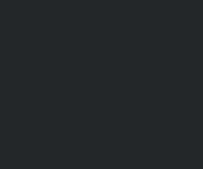
\includegraphics[scale=1]{process/img/1.png}
  \caption{进程创建、退出测试}
\end{figure}


在上图中,我们可以看到在我们输入\texttt{execk test}命令后,第一个模块起始为 \texttt{exec\_from\_kernel():begin}和\texttt{exec\_from\_kernel():end} ,在这之中完成了进程的创建,我们可以看到\texttt{execk return with 0}的返回值,这表明进程成功创建了。第二个模块起始为\texttt{runprog()},进入了内核进程的执行函数,我们可以看到\texttt{excute task pid = 2}说明进程现在正在执行,此后,我们可以看到一系列有关\texttt{pc\_exited()}的操作,说明当前内核进程已经执行完毕,正在退出。在最后我设置打印出了所有进程链表中的信息,我们可以看到存在一个状态为\texttt{TASK\_EXITED}的进程,表示进程已退出完毕。(在打印操作后会将进程移出所有进程链表)。



\texttt{execprio 进程优先级}

 

\begin{figure}[H]
  \centering
  \includegraphics[scale=1]{process/img/2.png}
  \caption{进程创建、退出测试}
\end{figure}


为了测试进程创建功能,我们提供了\texttt{execprio 进程优先级}测试指令。该指令的执行会在系统中新建一个进程,并且进程名即为输入指令后面的参数。测试结果照片如上。我们可以看到在我们输入\texttt{execprio 20}命令后,第一个模块以结束\texttt{exec\_from\_kernel():end} ,在这之中完成了进程的创建。第二个模块起始为\texttt{runprog()},进入了内核进程的执行函数,我们可以看到\texttt{current\_task: 2}的多次输出说明进程现在正在执行,此后,我们可以看到一系列有关\texttt{pc\_exited()}的操作,说明当前内核进程已经执行完毕,正在退出。(这是第一个版本的图片,因而打印输出和前图有所不同)

\subsection{进程调度测试}

为了测试多级就绪队列,看出它的动态更新优先级时间片,我们连续创建两个优先级相同的进程,查看测试结果。测试结果图片如下。

 
\begin{figure}[H]
  \centering
  \includegraphics[scale=1]{process/img/3.png}
  \caption{进程调度测试}
\end{figure}


首先,我们使用\texttt{execprio 4}两次,以创建两个name为\texttt{Process4}的进程。在图中第一部分是第二次优先级为4的进程执行结束,我们立即输入ps来打印所有进程链表信息,可以看到两个初始优先级都为4的进程都已完成执行,并退出。但是两个进程现在呈现的优先级已经不相同,并且具有不同的时间片。说明在调度执行的过程中,优先级和时间片确在动态更新。

\subsection{kill进程测试}

为了测试进程创建功能,我们提供了\texttt{kill 进程pid}测试指令。该指令的执行会在系统中新建一个进程,并且进程名即为输入指令后面的参数。测试结果照片如下。

 

\begin{figure}[H]
  \centering
  \includegraphics[scale=1]{process/img/4.png}
  \caption{kill进程测试}
\end{figure}

首先我们输入ps指令,以确保pid = 3的进程仍然在就绪队列中。如上图所示,此时该进程确实仍存在于系统之中,且处于就绪状态。然后我们输入\texttt{kill 3}指令,之后再次输入ps指令,从上图中可以看到,此时该进程已经不再存在于系统之中,这表明该进程已经成功被kill掉了。



\section{进程管理:UC/OS II}

\subsection{进程创建与退出测试}

\texttt{execk 进程名}

\begin{figure}[H]
  \centering
  \includegraphics[scale=0.6]{process/img/5.png}
  \caption{进程创建测试}
\end{figure}

在初始化后,我们可以使用\texttt{ps}命令,展示当前所有链表信息和任务就绪表的全部内容。我们可以看到仅IDLE进程(优先级数值为63)在任务就绪表中为\texttt{TASK\_TURE}。而其他优先级都为\texttt{TASK\_FALSE}。

\subsection{进程调度}

\begin{figure}[H]
  \centering
  \includegraphics[scale=0.6]{process/img/6.png}
  \caption{进程调度测试}
  \label{process-img-6}
\end{figure}


首先,我们使用了\texttt{execk test}创建了一个进程,在系统中分配了一个空闲的优先级53给新进程。进程创建后,我们立即打印了当前所有链表信息,和任务就绪表的全部内容。可以看到处于就绪表中的进程53和63在表中的状态是\texttt{TASK\_TURE},如图\ref{process-img-6}。

\begin{figure}[H]
  \centering
  \includegraphics[scale=0.6]{process/img/7.png}
  \caption{进程调度测试}
  \label{process-img-7}
\end{figure}

此时进程的优先级数值上高于kernel进程,但实际优先级意义上低于kernel进程,当kernel进程的时间片用完时,该进程被立即执行,再一次打印输出任务就绪表的全部内容,则显示该进程已不在就绪表中,如图\ref{process-img-7}。


\section{进程管理: 多级反馈队列}

\subsection{进程创建与退出测试}

\texttt{execk 进程名}

为了测试进程创建功能,我们提供了\texttt{execk 进程名}测试指令。该指令的执行会在系统中新建一个进程,并且进程名即为输入指令后面的参数。测试结果照片如下。

\begin{figure}[H]
  \centering
  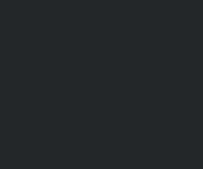
\includegraphics[scale=1]{process/img/1.png}
  \caption{进程创建、退出测试}
\end{figure}


在上图中,我们可以看到在我们输入\texttt{execk test}命令后,第一个模块起始为 \texttt{exec\_from\_kernel():begin}和\texttt{exec\_from\_kernel():end} ,在这之中完成了进程的创建,我们可以看到\texttt{execk return with 0}的返回值,这表明进程成功创建了。第二个模块起始为\texttt{runprog()},进入了内核进程的执行函数,我们可以看到\texttt{excute task pid = 2}说明进程现在正在执行,此后,我们可以看到一系列有关\texttt{pc\_exited()}的操作,说明当前内核进程已经执行完毕,正在退出。在最后我设置打印出了所有进程链表中的信息,我们可以看到存在一个状态为\texttt{TASK\_EXITED}的进程,表示进程已退出完毕。(在打印操作后会将进程移出所有进程链表)。



\texttt{execprio 进程优先级}

 

\begin{figure}[H]
  \centering
  \includegraphics[scale=1]{process/img/2.png}
  \caption{进程创建、退出测试}
\end{figure}


为了测试进程创建功能,我们提供了\texttt{execprio 进程优先级}测试指令。该指令的执行会在系统中新建一个进程,并且进程名即为输入指令后面的参数。测试结果照片如上。我们可以看到在我们输入\texttt{execprio 20}命令后,第一个模块以结束\texttt{exec\_from\_kernel():end} ,在这之中完成了进程的创建。第二个模块起始为\texttt{runprog()},进入了内核进程的执行函数,我们可以看到\texttt{current\_task: 2}的多次输出说明进程现在正在执行,此后,我们可以看到一系列有关\texttt{pc\_exited()}的操作,说明当前内核进程已经执行完毕,正在退出。(这是第一个版本的图片,因而打印输出和前图有所不同)

\subsection{进程调度测试}

为了测试多级就绪队列,看出它的动态更新优先级时间片,我们连续创建两个优先级相同的进程,查看测试结果。测试结果图片如下。

 
\begin{figure}[H]
  \centering
  \includegraphics[scale=1]{process/img/3.png}
  \caption{进程调度测试}
\end{figure}


首先,我们使用\texttt{execprio 4}两次,以创建两个name为\texttt{Process4}的进程。在图中第一部分是第二次优先级为4的进程执行结束,我们立即输入ps来打印所有进程链表信息,可以看到两个初始优先级都为4的进程都已完成执行,并退出。但是两个进程现在呈现的优先级已经不相同,并且具有不同的时间片。说明在调度执行的过程中,优先级和时间片确在动态更新。

\subsection{kill进程测试}

为了测试进程创建功能,我们提供了\texttt{kill 进程pid}测试指令。该指令的执行会在系统中新建一个进程,并且进程名即为输入指令后面的参数。测试结果照片如下。

 

\begin{figure}[H]
  \centering
  \includegraphics[scale=1]{process/img/4.png}
  \caption{kill进程测试}
\end{figure}

首先我们输入ps指令,以确保pid = 3的进程仍然在就绪队列中。如上图所示,此时该进程确实仍存在于系统之中,且处于就绪状态。然后我们输入\texttt{kill 3}指令,之后再次输入ps指令,从上图中可以看到,此时该进程已经不再存在于系统之中,这表明该进程已经成功被kill掉了。



\section{进程管理:UC/OS II}

\subsection{进程创建与退出测试}

\texttt{execk 进程名}

\begin{figure}[H]
  \centering
  \includegraphics[scale=0.6]{process/img/5.png}
  \caption{进程创建测试}
\end{figure}

在初始化后,我们可以使用\texttt{ps}命令,展示当前所有链表信息和任务就绪表的全部内容。我们可以看到仅IDLE进程(优先级数值为63)在任务就绪表中为\texttt{TASK\_TURE}。而其他优先级都为\texttt{TASK\_FALSE}。

\subsection{进程调度}

\begin{figure}[H]
  \centering
  \includegraphics[scale=0.6]{process/img/6.png}
  \caption{进程调度测试}
  \label{process-img-6}
\end{figure}


首先,我们使用了\texttt{execk test}创建了一个进程,在系统中分配了一个空闲的优先级53给新进程。进程创建后,我们立即打印了当前所有链表信息,和任务就绪表的全部内容。可以看到处于就绪表中的进程53和63在表中的状态是\texttt{TASK\_TURE},如图\ref{process-img-6}。

\begin{figure}[H]
  \centering
  \includegraphics[scale=0.6]{process/img/7.png}
  \caption{进程调度测试}
  \label{process-img-7}
\end{figure}

此时进程的优先级数值上高于kernel进程,但实际优先级意义上低于kernel进程,当kernel进程的时间片用完时,该进程被立即执行,再一次打印输出任务就绪表的全部内容,则显示该进程已不在就绪表中,如图\ref{process-img-7}。


\section{进程管理: 多级反馈队列}

\subsection{进程创建与退出测试}

\texttt{execk 进程名}

为了测试进程创建功能,我们提供了\texttt{execk 进程名}测试指令。该指令的执行会在系统中新建一个进程,并且进程名即为输入指令后面的参数。测试结果照片如下。

\begin{figure}[H]
  \centering
  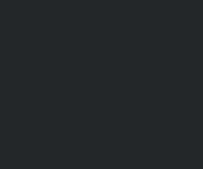
\includegraphics[scale=1]{process/img/1.png}
  \caption{进程创建、退出测试}
\end{figure}


在上图中,我们可以看到在我们输入\texttt{execk test}命令后,第一个模块起始为 \texttt{exec\_from\_kernel():begin}和\texttt{exec\_from\_kernel():end} ,在这之中完成了进程的创建,我们可以看到\texttt{execk return with 0}的返回值,这表明进程成功创建了。第二个模块起始为\texttt{runprog()},进入了内核进程的执行函数,我们可以看到\texttt{excute task pid = 2}说明进程现在正在执行,此后,我们可以看到一系列有关\texttt{pc\_exited()}的操作,说明当前内核进程已经执行完毕,正在退出。在最后我设置打印出了所有进程链表中的信息,我们可以看到存在一个状态为\texttt{TASK\_EXITED}的进程,表示进程已退出完毕。(在打印操作后会将进程移出所有进程链表)。



\texttt{execprio 进程优先级}

 

\begin{figure}[H]
  \centering
  \includegraphics[scale=1]{process/img/2.png}
  \caption{进程创建、退出测试}
\end{figure}


为了测试进程创建功能,我们提供了\texttt{execprio 进程优先级}测试指令。该指令的执行会在系统中新建一个进程,并且进程名即为输入指令后面的参数。测试结果照片如上。我们可以看到在我们输入\texttt{execprio 20}命令后,第一个模块以结束\texttt{exec\_from\_kernel():end} ,在这之中完成了进程的创建。第二个模块起始为\texttt{runprog()},进入了内核进程的执行函数,我们可以看到\texttt{current\_task: 2}的多次输出说明进程现在正在执行,此后,我们可以看到一系列有关\texttt{pc\_exited()}的操作,说明当前内核进程已经执行完毕,正在退出。(这是第一个版本的图片,因而打印输出和前图有所不同)

\subsection{进程调度测试}

为了测试多级就绪队列,看出它的动态更新优先级时间片,我们连续创建两个优先级相同的进程,查看测试结果。测试结果图片如下。

 
\begin{figure}[H]
  \centering
  \includegraphics[scale=1]{process/img/3.png}
  \caption{进程调度测试}
\end{figure}


首先,我们使用\texttt{execprio 4}两次,以创建两个name为\texttt{Process4}的进程。在图中第一部分是第二次优先级为4的进程执行结束,我们立即输入ps来打印所有进程链表信息,可以看到两个初始优先级都为4的进程都已完成执行,并退出。但是两个进程现在呈现的优先级已经不相同,并且具有不同的时间片。说明在调度执行的过程中,优先级和时间片确在动态更新。

\subsection{kill进程测试}

为了测试进程创建功能,我们提供了\texttt{kill 进程pid}测试指令。该指令的执行会在系统中新建一个进程,并且进程名即为输入指令后面的参数。测试结果照片如下。

 

\begin{figure}[H]
  \centering
  \includegraphics[scale=1]{process/img/4.png}
  \caption{kill进程测试}
\end{figure}

首先我们输入ps指令,以确保pid = 3的进程仍然在就绪队列中。如上图所示,此时该进程确实仍存在于系统之中,且处于就绪状态。然后我们输入\texttt{kill 3}指令,之后再次输入ps指令,从上图中可以看到,此时该进程已经不再存在于系统之中,这表明该进程已经成功被kill掉了。



\section{进程管理:UC/OS II}

\subsection{进程创建与退出测试}

\texttt{execk 进程名}

\begin{figure}[H]
  \centering
  \includegraphics[scale=0.6]{process/img/5.png}
  \caption{进程创建测试}
\end{figure}

在初始化后,我们可以使用\texttt{ps}命令,展示当前所有链表信息和任务就绪表的全部内容。我们可以看到仅IDLE进程(优先级数值为63)在任务就绪表中为\texttt{TASK\_TURE}。而其他优先级都为\texttt{TASK\_FALSE}。

\subsection{进程调度}

\begin{figure}[H]
  \centering
  \includegraphics[scale=0.6]{process/img/6.png}
  \caption{进程调度测试}
  \label{process-img-6}
\end{figure}


首先,我们使用了\texttt{execk test}创建了一个进程,在系统中分配了一个空闲的优先级53给新进程。进程创建后,我们立即打印了当前所有链表信息,和任务就绪表的全部内容。可以看到处于就绪表中的进程53和63在表中的状态是\texttt{TASK\_TURE},如图\ref{process-img-6}。

\begin{figure}[H]
  \centering
  \includegraphics[scale=0.6]{process/img/7.png}
  \caption{进程调度测试}
  \label{process-img-7}
\end{figure}

此时进程的优先级数值上高于kernel进程,但实际优先级意义上低于kernel进程,当kernel进程的时间片用完时,该进程被立即执行,再一次打印输出任务就绪表的全部内容,则显示该进程已不在就绪表中,如图\ref{process-img-7}。




\chapter{讨论及体会}

我实现的是内存部分。一开始看助教的代码,觉得内存部分已经实现的比较好了。尤其是虚拟内存部分,我觉得我在助教的基础上拓展一下,发挥一下,站在巨人的肩膀上总是好行事的。

所以把目标定在了页置换算法和内存池上。写好内存池之后才细看助教的代码,然后发现助教的TLB是有问题的。问题具体体现在无法真正映射虚拟内存。那内存池和页置换之前就要修复助教的BUG。

在修复助教的BUG的时候,发现一个底层的BUG,当系统处理异常的时候,他有时会跳转到\texttt{TLB\_refilling}异常。我觉得是硬件底层的问题。询问了另一个硬件小组的同学,他也这么觉得。

事情变得神秘了起来。我就把目标定在了使用红黑树管理\texttt{mm\_struct}中的\texttt{vma\_struct}和绕过TLB,写一个直接对vma层面操作的malloc和free函数。之所以写malloc/free也是为了验收的时候可以展示。同时这个malloc/free也给了之后版本的可拓展性。

说到可拓展性,VMA里面的合并接口,我都留了出来,假如之后可以再写页置换的话,还可以再写一写。

其他方面,比如像时间安排啥的。我都没什么问题,慢慢写的,也不紧张。但是没有地方可以调试是一个问题。实验室总是不开门,写到一定程度是一定要去实验室测试代码的。所以还是希望之后实验室能多开门。

最后,这个操作系统还是极大的提高了我的视野,我才知道硬件小组的人都这么强。可能只有强者才能学硬件。

~\hfill 李仁钟

\newpage
我实现的是内存部分。一开始看助教的代码,觉得内存部分已经实现的比较好了。尤其是虚拟内存部分,我觉得我在助教的基础上拓展一下,发挥一下,站在巨人的肩膀上总是好行事的。

所以把目标定在了页置换算法和内存池上。写好内存池之后才细看助教的代码,然后发现助教的TLB是有问题的。问题具体体现在无法真正映射虚拟内存。那内存池和页置换之前就要修复助教的BUG。

在修复助教的BUG的时候,发现一个底层的BUG,当系统处理异常的时候,他有时会跳转到\texttt{TLB\_refilling}异常。我觉得是硬件底层的问题。询问了另一个硬件小组的同学,他也这么觉得。

事情变得神秘了起来。我就把目标定在了使用红黑树管理\texttt{mm\_struct}中的\texttt{vma\_struct}和绕过TLB,写一个直接对vma层面操作的malloc和free函数。之所以写malloc/free也是为了验收的时候可以展示。同时这个malloc/free也给了之后版本的可拓展性。

说到可拓展性,VMA里面的合并接口,我都留了出来,假如之后可以再写页置换的话,还可以再写一写。

其他方面,比如像时间安排啥的。我都没什么问题,慢慢写的,也不紧张。但是没有地方可以调试是一个问题。实验室总是不开门,写到一定程度是一定要去实验室测试代码的。所以还是希望之后实验室能多开门。

最后,这个操作系统还是极大的提高了我的视野,我才知道硬件小组的人都这么强。可能只有强者才能学硬件。

~\hfill 李仁钟

\newpage
我实现的是内存部分。一开始看助教的代码,觉得内存部分已经实现的比较好了。尤其是虚拟内存部分,我觉得我在助教的基础上拓展一下,发挥一下,站在巨人的肩膀上总是好行事的。

所以把目标定在了页置换算法和内存池上。写好内存池之后才细看助教的代码,然后发现助教的TLB是有问题的。问题具体体现在无法真正映射虚拟内存。那内存池和页置换之前就要修复助教的BUG。

在修复助教的BUG的时候,发现一个底层的BUG,当系统处理异常的时候,他有时会跳转到\texttt{TLB\_refilling}异常。我觉得是硬件底层的问题。询问了另一个硬件小组的同学,他也这么觉得。

事情变得神秘了起来。我就把目标定在了使用红黑树管理\texttt{mm\_struct}中的\texttt{vma\_struct}和绕过TLB,写一个直接对vma层面操作的malloc和free函数。之所以写malloc/free也是为了验收的时候可以展示。同时这个malloc/free也给了之后版本的可拓展性。

说到可拓展性,VMA里面的合并接口,我都留了出来,假如之后可以再写页置换的话,还可以再写一写。

其他方面,比如像时间安排啥的。我都没什么问题,慢慢写的,也不紧张。但是没有地方可以调试是一个问题。实验室总是不开门,写到一定程度是一定要去实验室测试代码的。所以还是希望之后实验室能多开门。

最后,这个操作系统还是极大的提高了我的视野,我才知道硬件小组的人都这么强。可能只有强者才能学硬件。

~\hfill 李仁钟



\chapter{组内成员分工}

本次课程设计分工情况安排如下

\begin{table}[H]
  \centering
  \caption{分工情况}
  \begin{tabular}{|l|l|l|}
    \hline
    角色 & 姓名 & 分工 \\
    \hline
    组长 & 陈翰逸 & 文件系统 \\
    \hline
    组员 & 李仁钟 & 内存部分 \\
    \hline
    组员 & 萧芷晴 & \makecell{进程管理 \\ 多级反馈进程调度 \\ uc/osII任务调度} \\
    \hline
    ~ & 共同参与 & \makecell{中期报告的参与部分的撰写 \\ 定期的组内讨论与交流} \\
    \hline
  \end{tabular}
\end{table}

\chapter{附注}


\chapter{参考文献}

???